% remember to set these at the start of each chapter
\chapter{Background} 
\label{background} 

\section{Neural Networks}

The term Neural Network (NN) refers to a computational model that is artificially built in computers. The artificial Neural Network is inspired by the way biological neural networks in the human brain process information. Artificial Neural Network is the most powerful Machine Learning model. Neural Networks are recognized for many breakthrough achievements in speech recognition, computer vision and text processing. In this section, we will discuss the fundamentals of a Neural Network.

\subsection{A Single Neuron}
Neuron, or node, is a basic computation unit in NN. It simply takes some inputs $\mathbf{x} = (x_0,...,x_i)$ and computes an output. Each input has an associated weight $(w_0,...,w_i)$, which is assigned on the basis of its relative importance to other inputs. The node applies a function $f$ to the weighted sum of its inputs (and a bias term $b$). The output of a node is $f(w_1x_1 +...+ w_ix_i + b)$, shown in Fig.\,\ref{node}.
\begin{figure}
	\centering
	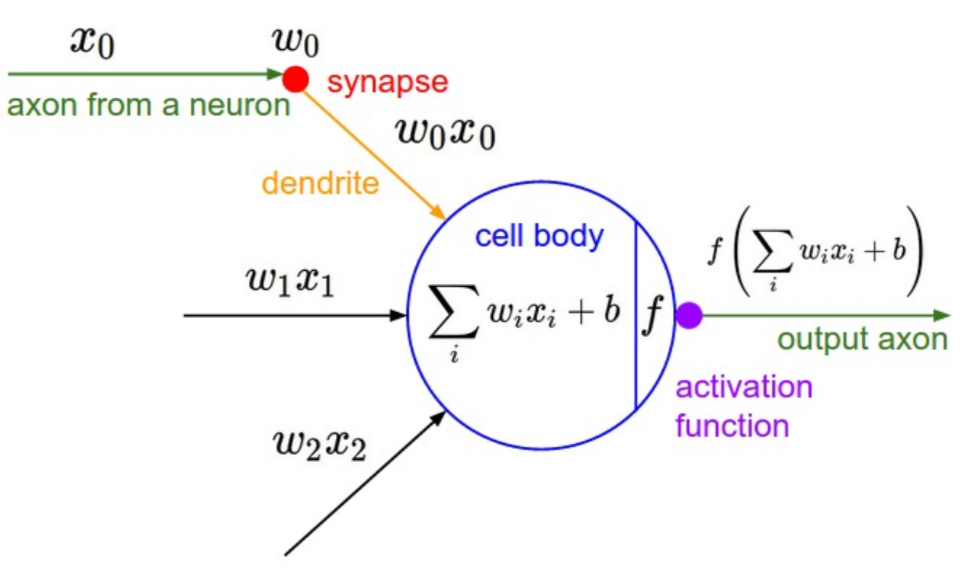
\includegraphics[scale=0.5]{Figs/node.png}
    \caption{A Node}
    \label{node}
\end{figure}

The function $f$ is non-linear and is called the Activation Function. The purpose of the activation function is to introduce non-linearity into the output of a node. The following activation function (Fig.\,\ref{activation}) is often used:
\begin{figure}
	\centering
	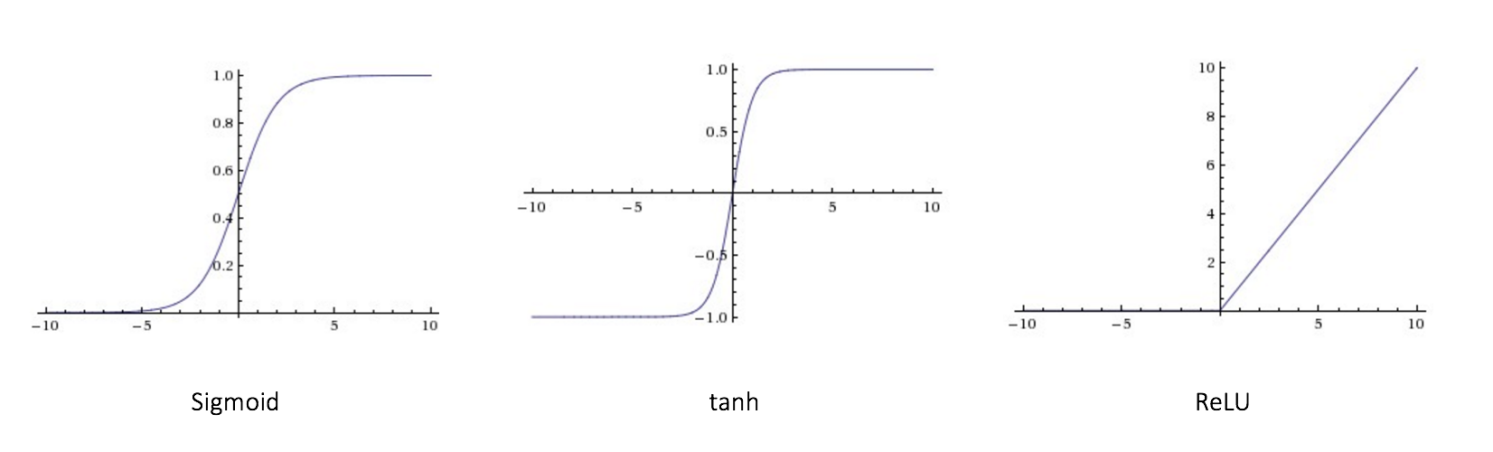
\includegraphics[scale=0.5]{Figs/activation.png}
    \caption{Activation Functions}
    \label{activation}
\end{figure}

\begin{itemize}
  \item Sigmoid: takes a real-valued input and squashes it to range between 0 and 1
        $$ \sigma(x) =  \frac{\mathrm{1} }{\mathrm{1} + e^{-x} }  $$ 
  \item tanh: takes a real-valued input and squashes it to the range [-1, 1]
        $$ tanh(x) = 2\cdot\sigma(2x)-1 $$
        
  \item ReLU(Rectified Linear Unit) \citep{Nair:2010:RLU:3104322.3104425}: takes a real-valued input and thresholds it at zero
        $$f(x) = \max(0,x)$$
\end{itemize}

\subsection{Feedforward Neural Network}

The simplest Neural Network is a feedforward fully connected network. It is formed by one or multiple layers of nodes. Nodes in adjacent layers have connections between them. A connection represents a set of weights.


\noindent An example of a two hidden layer feedforward neural network is shown in Fig.\,\ref{two_layer}.

\begin{figure}[h]
	\centering
	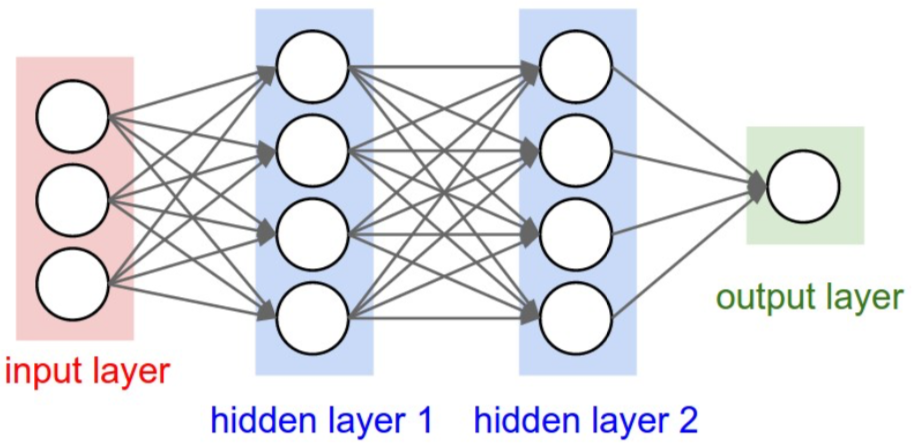
\includegraphics[scale=0.5]{Figs/2hidden.png}
    \caption{Feedforward Neural Network}
    \label{two_layer}
\end{figure}

\noindent A feedforward neural network can consist of three types of nodes:

\begin{enumerate}
\item Input Nodes – The Input nodes take in a input $\mathbf{x}$ in the form of vector $(x_0,...,x_i)$. These nodes are together referred to as the “Input Layer”. No computation is performed in any of the Input nodes – they just pass on the information to the hidden nodes.

\item Hidden Nodes – The Hidden nodes are in between Input Layer and Output Layer. They have no direct connection with the network input and the network output, thus they are called "Hidden" and form "Hidden Layer". After training, Hidden Node will learn some relationship (non-linearality) between its input and output. A feedforward network can have zero, one, or multiple Hidden Layers.

\item Output Nodes – The Output nodes are collectively referred to as the “Output Layer” and are responsible for computations and producing output from the "Hidden Layer". Output Layer works in similar way as a Hidden Layer, but the output of this layer is considered the final output of the network.

\end{enumerate}

In a feedforward network, the information moves in only one direction – forward – from the input nodes, through the hidden nodes and to the output nodes. There are no cycles or loops in the network.


\subsection{Multi Layer Perceptron}
A Multi Layer Perceptron (MLP) contains one or more hidden layers (apart from one input and one output layer). The capacity of the network increases with more hidden units and more hidden layers (Fig.\,\ref{anyfunction}). A multilayer perceptron with at least one hidden layer can represent any function \citep{Cybenko1989}.

\begin{figure}[h]
	\centering
	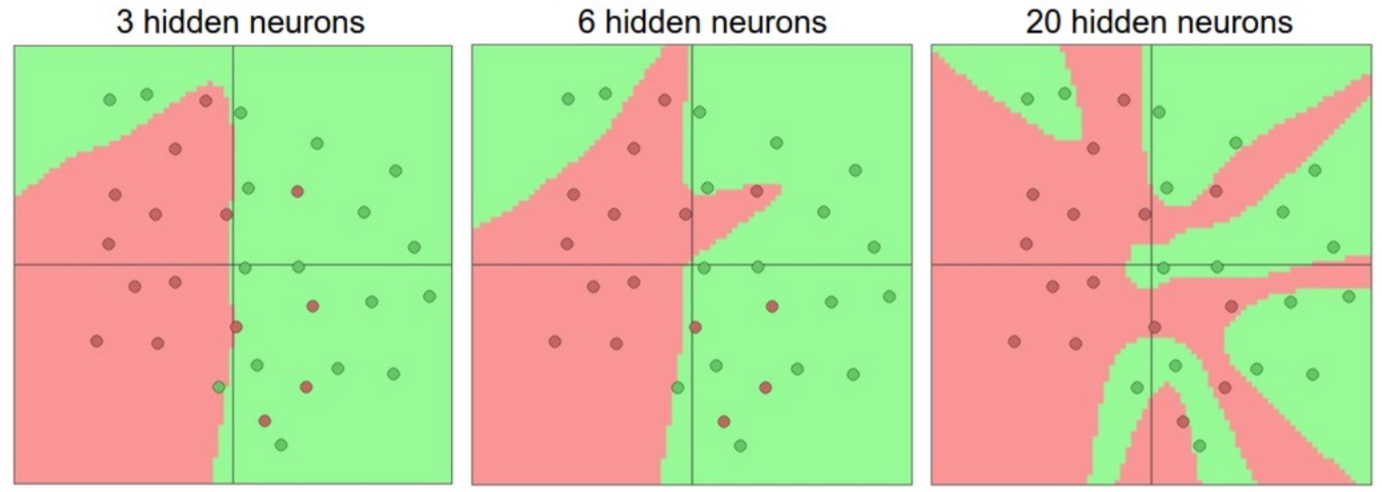
\includegraphics[scale=0.5]{Figs/anyfunction.png}
    \caption{Non-linear decision boundary}
    \label{anyfunction}
\end{figure}


Fig.\,\ref{one_layer} shows a multilayer perceptron with a single hidden layer. Each connection has a weight associated with it.

\begin{figure}[h]
	\centering
	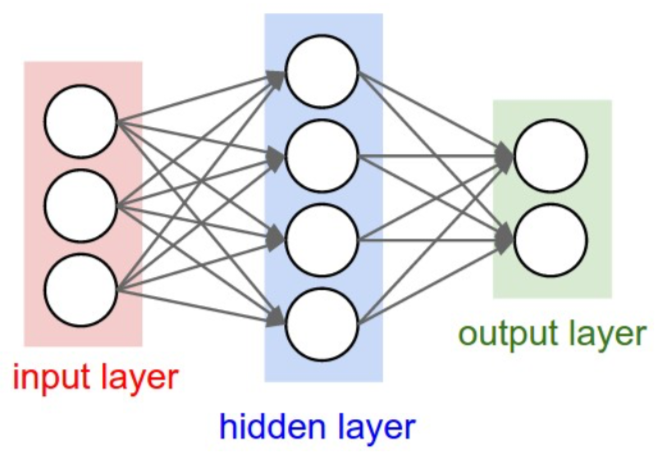
\includegraphics[scale=0.5]{Figs/1hidden.png}
    \caption{Feedforward Neural Network}
    \label{one_layer}
\end{figure}


\textbf{Input Layer}: The Input layer has three nodes. The Bias is omitted for simplicity but has a value of 1. The nodes take in the input $\mathbf{x} = (x_1,x_2,x_3)$. These values form the Input Layer and are passed to the Hidden layer with no computation.

\textbf{Hidden Layer}: The Hidden layer has four nodes. To distinguish from the output layer, here let $v$ denote a weight and $h$ denote the output of a neuron in hidden layer. $D$ denotes the number of inputs. The output of the $j$th neuron is $h_j(\mathbf{x}) = f(v_{j0}+\sum_{i=1}^{D=3} x_iv_{ji})$. $f$ is an activation function.

\textbf{Output Layer}: The Output layer has two nodes which take inputs from the Hidden layer and perform similar computations.
$w$ denote a weight and $o$ denote the output of a neuron in output layer. The output of the $k$th neuron is $o_k(\mathbf{x}) = g(w_{k0}+\sum_{j=1}^{J=4} h_j(\mathbf{x}) w_{kj})$. $g$ is also an activation function.

Given a set of features $\mathbf{x} = (x_1,...,x_n)$ and a target $\mathbf{t} = (t_1,..,t_n)$, a Multi Layer Perceptron can learn the relationship between the features and the target, for either classification or regression.

\newcommand{\argminE}{\mathop{\mathrm{argmin}}}  

\subsection{Forward and Backward Propagation}
There are two phases in the learning process, forward and backward. Forward phase is making output prediction from the given input.
Backward phase is backward propagation of errors. A Neural Network learns through Back-Propagation by calculating the error from the output $\mathbf{o}$ to the target value $\mathbf{t}$, then improving the weights in all nodes. The learning is "supervised", meaning the target value $\mathbf{t}$ must be given to the network respect to each input  $\mathbf{x}$ in training. The objective of learning is to get $\mathbf{w}^* = \argminE_\mathbf{w} \sum_{n=1}^N loss(\mathbf{o}^{(n)},\mathbf{t}^{(n)})$, where $\mathbf{o} = f(\mathbf{x};\mathbf{w})$ is the output of the network. With hidden units, this objective is not convex. We can minimize the function by gradient descent (no guarantees gradient methods would not end up in a local minima/saddle point, but experiments evidence that most local minimas are almost as good as the global minima).

A loss function $L$ measures the error between network output $\mathbf{o}$ and the target value $\mathbf{t}$. Let $E$ denote such error. For clarity, we can expand the output layer as shown in Fig.\,\ref{expand2}. $o_k$ is the output of unit $k$, $g$ is the output layer activation function, $z_{k}$ is the net input to output unit $k$, $w_{ki}$ is the weight from input $i$ to $k$. 
\begin{figure}[h]
	\centering
	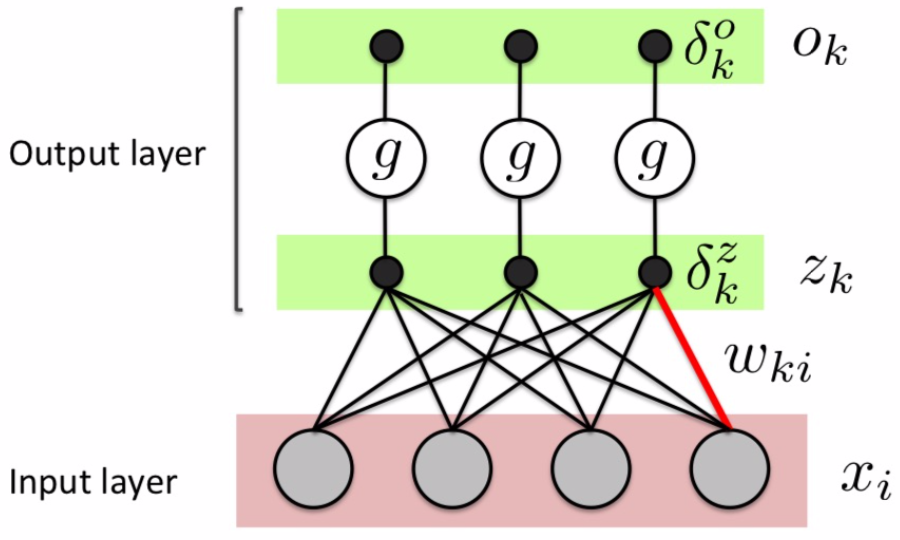
\includegraphics[scale=0.5]{Figs/singlelayer2.png}
    \caption{Single Layer Network}
    \label{expand2}
\end{figure}
Error gradients for single layer network is 
$$\frac{\partial E}{\partial w_{ki}} = 
    \frac{\partial E}{\partial o_{k}} 
    \frac{\partial o_{k}}{\partial z_{k}} 
    \frac{\partial z_{k}}{\partial w_{ki}} $$
Error at output $o_k$ is $\delta_k^o =  \frac{\partial E}{\partial o_{k}} $.
$$\frac{\partial E}{\partial w_{ki}} = 
    \frac{\partial E}{\partial o_{k}} 
    \frac{\partial o_{k}}{\partial z_{k}} 
    \frac{\partial z_{k}}{\partial w_{ki}} 
    =  
    \delta_k^o 
    \frac{\partial o_{k}}{\partial z_{k}} 
    \frac{\partial z_{k}}{\partial w_{ki}}  $$
Since $o_k = g(z_k)$, $$\delta_k^z = \delta_k^o \cdot \frac{\partial o_{k}}{\partial z_{k}}$$ then we have $$\frac{\partial E}{\partial w_{ki}} = \delta_k^z \frac{\partial z_{k}}{\partial w_{ki}} =  \delta_k^z \cdot x_i$$ 
Assuming the loss function is mean-squared error (MSE), on a single training example $n$, we have:
$$\frac{\partial E}{\partial o_k^{(n)}} = o_k^{(n)} - t_k^{(n)} := \delta_k^o$$Using logistic activation functions:$$ o_k^{(n)} = g(z_k^{(n)}) = (1 + \exp(-z_k^{(n)}))^{-1}$$
$$\frac{\partial o_k^{(n)}}{\partial z_k^{(n)}} = o_k^{(n)}(1-o_k^{(n)})$$
The error gradient is then:
$$\frac{\partial E}{\partial w_{ki}} =  \sum_{n=1}^N \frac{\partial E}{\partial o_{k}^{(n)}}\frac{\partial o_{k}^{(n)}}{\partial z_{k}^{(n)}} \frac{\partial z_{k}^{(n)}}{\partial w_{ki}} = \sum_{n=1}^N (o_k^{(n)} - t_k^{(n)})o_k^{(n)} (1-o_k^{(n)}) x_i^{(n)}$$
The gradient descent update rule is given by:
$$w_{ki} := w_{ki} - \eta \frac{\partial E}{\partial w_{ki}} = w_{ki} - \eta  \sum_{n=1}^N (o_k^{(n)} - t_k^{(n)})o_k^{(n)} (1-o_k^{(n)}) x_i^{(n)}$$
\begin{figure}[h]
	\centering
	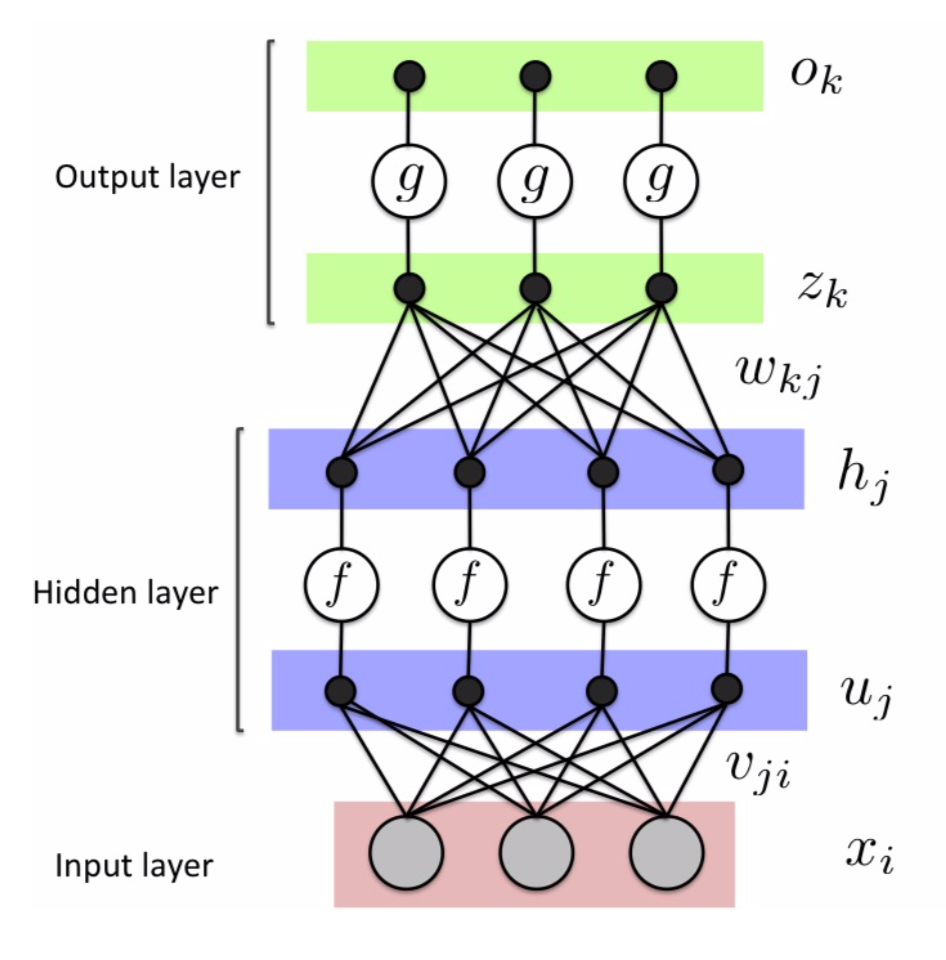
\includegraphics[scale=0.5]{Figs/multilayerbackprop.png}
    \caption{Multi Layer Network}
    \label{multi}
\end{figure}
where $\eta$ is a pre-defined learning rate. The output weight gradients for a multi-layer network are the same as for a single layer network (Fig.\,\ref{multi}):
$$\frac{\partial E}{\partial w_{kj}} =  \sum_{n=1}^N \frac{\partial E}{\partial o_{k}^{(n)}}\frac{\partial o_{k}^{(n)}}{\partial z_{k}^{(n)}} \frac{\partial z_{k}^{(n)}}{\partial w_{kj}} = \sum_{n=1}^N \delta_k^{z,(n)} h_j^{(n)}$$
where $\delta_k$ is the error w.r.t. the net input for unit $k$. Hidden weight gradients are then computed via back propagation:
$$\frac{\partial E}{\partial h_{j}^{(n)}} =  \sum_{k} \frac{\partial E}{\partial o_{k}^{(n)}}\frac{\partial o_{k}^{(n)}}{\partial z_{k}^{(n)}} \frac{\partial z_{k}^{(n)}}{\partial h_{j}^{(n)}} = \sum_{k} \delta_k^{z,(n)} w_{kj} := \delta_j^{h,(n)}$$
$$ \frac{\partial E}{\partial v_{ji}} 
= \sum_{n=1}^N \frac{\partial E}{\partial h_{j}^{(n)}}\frac{\partial h_{j}^{(n)}}{\partial u_{j}^{(n)}} \frac{\partial u_j^{(n)}}{\partial v_{ji}}
= \sum_{n=1}^N \delta_j^{h,(n)} f'(u_j^{(n)})\frac{\partial u_j^{(n)}}{\partial v_{ji}} 
= \sum_{n=1}^N \delta_j^{u,(n)} x_i^{(n)} $$

Often times, the learning rate $\eta$ is difficult to set. If it is too large, the local and global minima can be “overshot”, leading to slow convergence, and if the learning rate is too small, it can take a long time to converge to an acceptable minimum. “Adaptive Moment Estimation (Adam)” \citep{adam} optimizer was invented to adaptively set the learning rate during training.


\section{Convolutional Neural Networks}
A Convolutional Neural Network (CNN) (Fig.\,\ref{cnn}) is a Neural Network model which can take in an input image, assign importance (learnable weights and biases) to regions/groups of pixels via kernals/filters. The pre-processing required in a CNN is much lower as compared to other classification algorithms. While in primitive methods filters are hand-engineered, with enough training, CNNs have the ability to learn these kernals.
\begin{figure}[h]
	\centering
	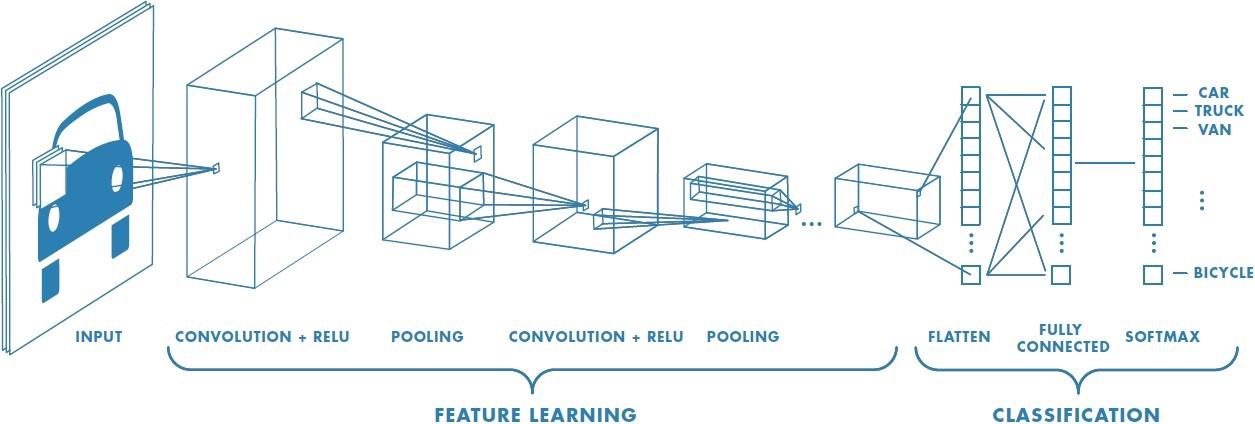
\includegraphics[width=\textwidth]{Figs/cnn.jpg}
    \caption{Convolutional Neural Network}
    \label{cnn}
\end{figure}

The architecture of a CNN is analogous to that of the connectivity pattern of Neurons in the Human Brain and was inspired by the organization of the Visual Cortex. Individual neurons respond to stimuli only in a restricted region of the visual field known as the Receptive Field. A collection of such fields overlap to cover the entire visual area.

\subsection{Convolution Layer — The Kernel}
A CNN is able to successfully capture the Spatial and Temporal dependencies in an image through the application of relevant kernels. The architecture performs a better fitting to the image dataset due to the reduction in the number of parameters involved and reusability of weights. In other words, the network can be trained to understand the sophistication of the image better.

Fig.\,\ref{kernels} shows four line detection kernels which respond maximally to horizontal, vertical and oblique (+45 and - 45 degree) single pixel wide lines.

\begin{figure}[h]
	\centering
	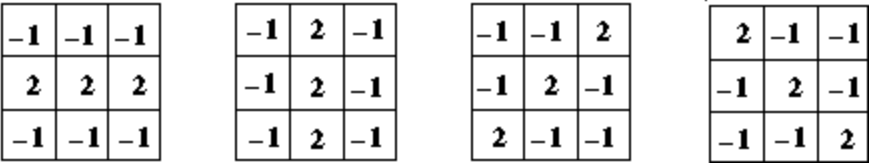
\includegraphics[scale=0.6]{Figs/kernels.png}
    \caption{Kernels}
    \label{kernels}
\end{figure}

Let K denote this kernel. Convolution is done by matrix multiplication operation between K and the portion P of the image over which the kernel is hovering. The kernel is moved from left to right, top to bottom with a certain Stride value. Figure * shows two steps of kernel application on image with Stride set to 1. 

CNN need not be limited to only one Convolutional Layer. Conventionally, the first ConvLayer is responsible for capturing the Low-Level features such as edges, color, gradient orientation, etc. With added layers, the architecture adapts to the High-Level features as well, giving us a network which has the wholesome understanding of images in the dataset.

\subsection{Pooling Layer}

Similar to the Convolutional Layer, the Pooling layer is responsible for reducing the spatial size of the Convolved Feature. This is to decrease the computational power required to process the data through dimensionality reduction. Furthermore, it is useful for extracting dominant features which are rotational and positional invariant, thus maintaining the process of effectively training of the model.

There are two types of Pooling: Max Pooling and Average Pooling. Max Pooling returns the maximum value from the portion of the image covered by the Kernel. On the other hand, Average Pooling returns the average of all the values from the portion of the image covered by the Kernel.

Max Pooling also performs as a Noise Suppressant. It discards the noisy activations altogether and also performs de-noising along with dimensionality reduction. On the other hand, Average Pooling simply performs dimensionality reduction as a noise suppressing mechanism. 

The Convolutional Layer and the Pooling Layer, together form the i-th layer of a Convolutional Neural Network. Depending on the complexities in the images, the number of such layers may be increased for capturing low-levels details even further, but the more layers CNN has the more computation it performs.

\subsection{Classification — Fully Connected Layer (FC Layer)}

Fully-Connected layer is used to learn non-linear combinations of the high-level features as represented by the output of the convolutional layer. The Fully-Connected layer is learning a possibly non-linear function in that space.

Now that we have converted our input image into a suitable form for our Multi-Level Perceptron, we shall flatten the image into a column vector. The flattened output is fed to a feed-forward neural network and backpropagation applied to every iteration of training. Over a series of epochs, the model is able to distinguish between dominating and certain low-level features in images and classify them using the Softmax activation function.

\section{K-Fold Cross Validation}
K-Fold Cross Validation \citep{Kohavi95astudy} (Fig.\,\ref{kfold}) is where a given data set is split into a K number of sections/folds where each fold is used as a testing set at some point. Lets take the scenario of 5-Fold cross validation(K=5). Here, the data set is split into 5 folds. In the first iteration, the first fold is used to test the model and the rest are used to train the model. In the second iteration, 2nd fold is used as the testing set while the rest serve as the training set. This process is repeated until each fold of the 5 folds have been used as the testing set. The advantage of this method over repeated random sub-sampling is that all observations are used for both training and validation, and each observation is used for validation exactly once. The testing accuracy of each fold will be averaged to evaluate the model's performance. 

\begin{figure}[h]
	\centering
	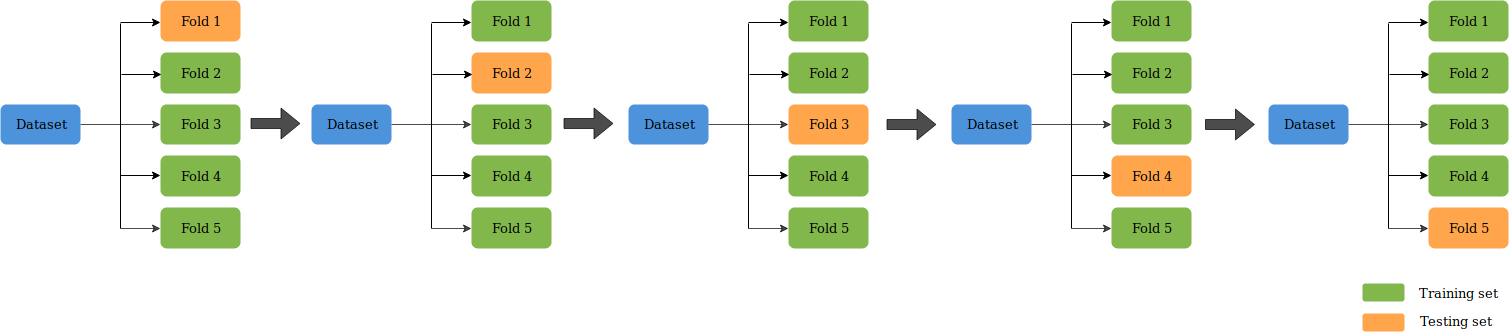
\includegraphics[width=\textwidth]{Figs/kfold.png}
    \caption{5-Fold Cross Validation}
    \label{kfold}
\end{figure}


\section{Image data augmentation}

The performance of deep learning neural networks often improves with the amount of data available. Data augmentation is a technique to artificially create new training data from existing training data \citep{Mikolajczyk2018}. This is done by applying domain-specific techniques to examples from the training data that create new and different training examples.

\begin{figure}[h]
	\centering
	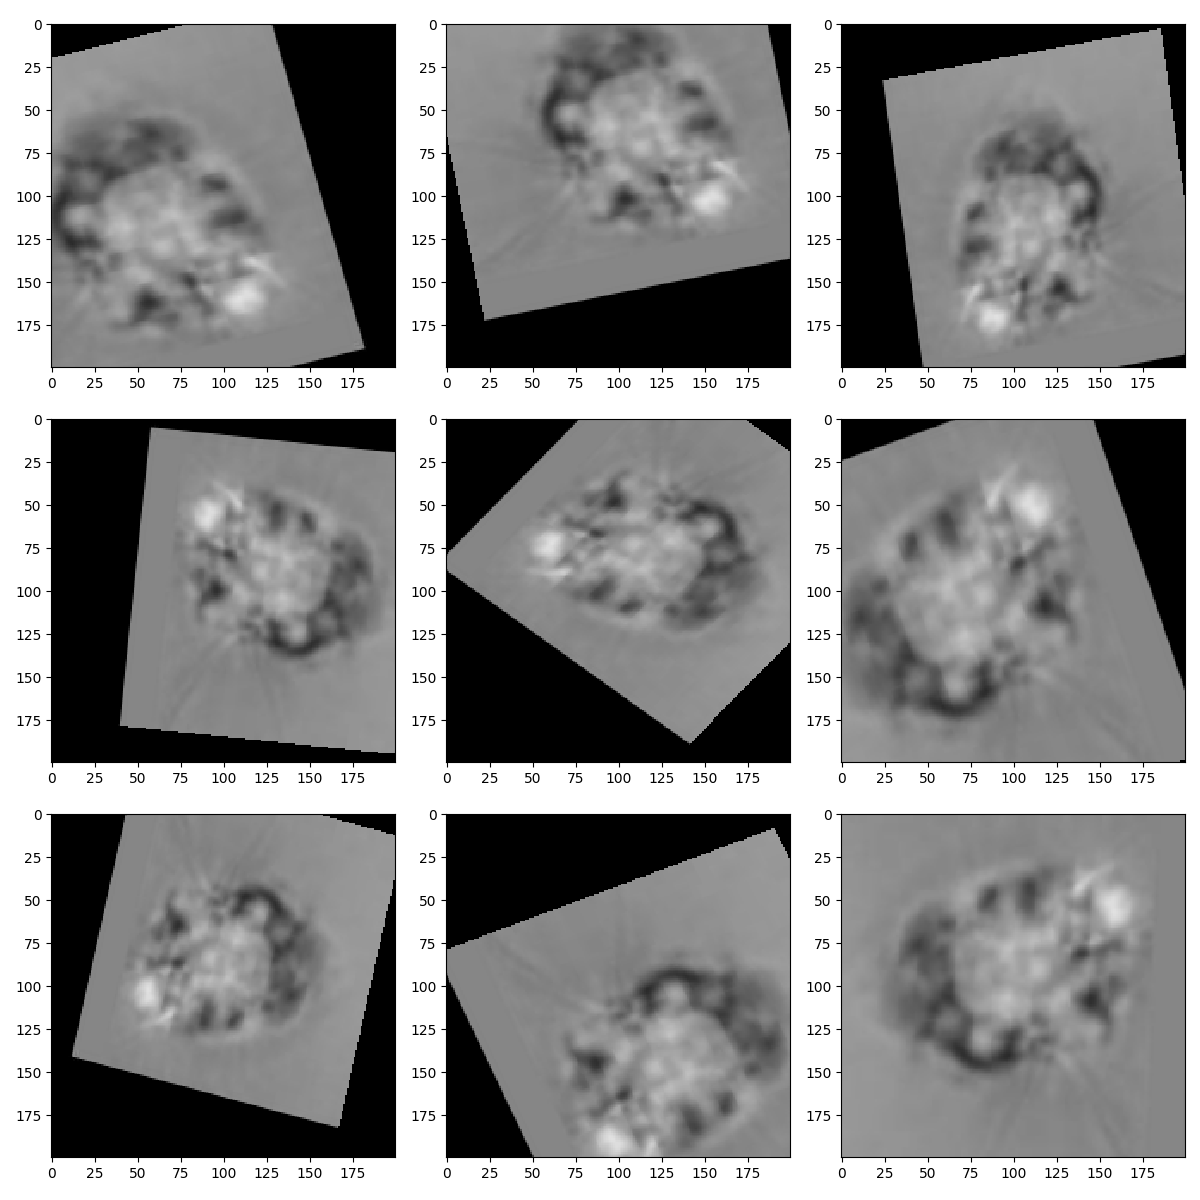
\includegraphics[width=.5\textwidth]{Figs/dataaug.jpg}
    \caption{Image Data Augmentation}
    \label{dataaug}
\end{figure}

Image data augmentation (Fig.\,\ref{dataaug}) is to create transformed versions of images in the training dataset that belong to the same class as the original image. Transforms include a range of operations from the field of image manipulation, such as shifts, flips, zooms, crops.

Convolutional neural network can learn features that are invariant to their location in the image. Image augmentation can further aid in this transform invariant approach to learning and can aid the model in learning features that are also invariant to transforms such as left-to-right to top-to-bottom ordering. Image data augmentation is typically only applied to the training dataset, and not to the validation or test dataset. 



